\documentclass{article}
 
% Load the package
\usepackage{tikz}

\usetikzlibrary{
    arrows,
    backgrounds,
    calc,
    chains,
    decorations.pathreplacing,
    decorations.pathmorphing,
    matrix,
    %node-families,
    positioning,
    %positioning-plus,
    shapes,
    shapes.geometric,
    shapes.symbols,
    topaths,
    trees,
}

 
\begin{document}

\tikzstyle{texto} = [above, text width=6em, text centered]
% \newcommand{\fourup}[5]{%
%   \begin{pgfonlayer}{background}
%     % Left-top corner of the background rectangle
%     \path (#1.west |- #2.north)+(-0.5,0.5) node (a1) {};
%     % Right-bottom corner of the background rectanle
%     \path (#3.east |- #4.south)+(+0.5,-0.25) node (a2) {};
%     % Draw the background
%     \path[fill=yellow!20,rounded corners, draw=black!50, dashed]
%       (a1) rectangle (a2);
%     \path (a1.east |- a1.south)+(0.8,-0.3) node (u1)[texto]
%       {\scriptsize\textit{#5}};
%   \end{pgfonlayer}}
%   \newcommand{\threeup}[4]{%
%   \begin{pgfonlayer}{background}
%     % Left-top corner of the background rectangle
%     \path (#1.west |- #2.north)+(-0.5,0.5) node (a1) {};
%     % Right-bottom corner of the background rectanle
%     \path (#2.east |- #3.south)+(+0.5,-0.25) node (a2) {};
%     % Draw the background
%     \path[fill=yellow!20,rounded corners, draw=black!50, dashed]
%       (a1) rectangle (a2);
%     \path (a1.east |- a1.south)+(0.8,-0.3) node (u1)[texto]
%       {\scriptsize\textit{#4}};
%   \end{pgfonlayer}}
%   \newcommand{\twoup}[3]{%
%   \begin{pgfonlayer}{background}
%     % Left-top corner of the background rectangle
%     \path (#1.west |- #2.north)+(-0.5,0.5) node (a1) {};
%     % Right-bottom corner of the background rectanle
%     \path (#1.east |- #2.south)+(+0.5,-0.25) node (a2) {};
%     % Draw the background
%     \path[fill=yellow!20,rounded corners, draw=black!50, dashed]
%       (a1) rectangle (a2);
%     \path (a1.east |- a1.south)+(0.8,-0.3) node (u1)[texto]
%       {\scriptsize\textit{#3}};
%   \end{pgfonlayer}}

%%%%%%%%%%%%%%%%%%%%%%%%%%%%%%%%%%%%%
\section*{Introduction}

\renewcommand{\dots}{\ \dotfill{}\ } 
\newcommand{\command}[2]{#1~\dotfill{}~#2\\} 
\newcommand{\defin}[2]{#1~\dotfill{}~#2\\} 

\subsection{Graph maths}

\defin{Graph}{$G=(N,E)$}

\subsection{Graph implementations}
			
\subsection{Graph Algorithms}
			
\defin{BFS}{Breadth-first search}
\defin{DFS}{Depth-first search}
\defin{Random Walk}{randomize decision to follow edges}
\defin{Biased 2nd order Random Walk}{randomize decision to follow edges}

\subsection{Graph ML concepts}

\defin{note2vec}{Use flexible, biased random walks that can trade off between local and global views of the network\cite{grovlesk16}}
\defin{deepwalk}{...}

\subsection{Maths stuff}

\defin{Real numbers}{R}
\defin{Integers}{Z}

\subsection{Machine Learning concepts}

\defin{Stochastic Gradient Descent}{evaluate gradients for each individual training example}

\subsection{Machine Learning functions}

\defin{SoftMax}{$\sigma(z_i) = \frac{e^{z_{i}}}{\sum_{j=1}^K e^{z_{j}}} \ \ \ for\ i=1,2,\dots,K$}
\defin{Sigmoid}{$\sigma(z) = \frac{1} {1 + e^{-z}}$}
\defin{Relu}{$Relu(z) = max(0, z)$}
\defin{Mean Absolute Error (MAE)}{$\sum_{i=1}^{D}|x_i-y_i|$}
\defin{Mean Squared Error (MSE)}{$\sum_{i=1}^{D}(x_i-y_i)^2$}
%\defin{Huber loss}{$L_{\delta}=
%    \left\{\begin{matrix}
%        \frac{1}{2}(y - \hat{y})^{2} & if \left | (y - \hat{y})  \right | < \delta\\
%        \delta ((y - \hat{y}) - \frac1 2 \delta) & otherwise
%    \end{matrix}\right.$}
\defin{Cross Entropy}{$-{(y\log(p) + (1 - y)\log(1 - p))}$ for $M = 2$ \\ $-\sum_{c=1}^My_{o,c}\log(p_{o,c})$ for $M > 2$}    
					
\subsection{Statistics}

%\begin{tabular}{c >{\bfseries}r @{\hspace{0.7em}}c @{\hspace{0.4em}}c @{\hspace{0.7em}}l}
 % \multirow{10}{*}{\rotatebox{90}{\parbox{1.1cm}{\bfseriescentering actual value}}} & 
%    & \multicolumn{2}{c}{\bfseries Prediction outcome} & 
%  & & \bfseries p & \bfseries n & \bfseries total 
%  & p$'$ & \MyBox{True}{Positive} & \MyBox{False}{Negative} & P$'$ [2.4em]
%  & n$'$ & \MyBox{False}{Positive} & \MyBox{True}{Negative} & N$'$ 
%  & total & P & N &
%\end{tabular}

\defin{True Positive}{$TP$}
\defin{False Positive}{$FP$}
\defin{True Negative}{$TN$}
\defin{False Negative}{$FN$}
\defin{Precision}{$\frac{TP}{TP+FP}$}
\defin{Recall}{$\frac{TP}{TP+FN}$}
\defin{Accuracy}{$\frac{TP+TN}{TP+TN+FP+FN}$}
\defin{Sensitivity = Recall}{$\frac{TP}{TP+FN}$}
\defin{Specificity}{$\frac{TN}{FP+TN}$}
\defin{Cosine similarity}{$Cosine(x,y) = \frac{x \cdot y}{|x||y|}$}
\defin{Jaccard similarity}{$Jaccard(U,V) = \frac{|U \cap V|}{|U \cup V|}$}
\defin{Pointwise Mutual Information (PMI) similarity}{$PMI(x;y) = \log{\frac{p(x,y)}{p(x)p(y)}}$}


\section{Over-smoothing}

This problem happens when we stack too many layers in a GNN. The 
problem is that the embeddings tend to converge to a similar value. 
But we want node embeddings to be different.

The problem is that as we go out from the node of interest, the number of 
shared nodes also goes up. The embedding of a node is determined by the \emph{receptive field}. A receptive field is a set of nodes that are connected to the node of interest. If two nodes have highly overlapping receptive fields, then the embeddings will be likewise very similar. This results in the over-smoothing problem.

\subsubsection{Layers}

We need to be careful we don't have too many layers. A too deep network will result in oversmoothing. Setting the number of layers to be only slightly more than the size of the receptive field is a good first approximation.

\subsubsection{Increase expressive power}

One approach is to increase expressive power with each layer.

\begin{figure*}[ht]
    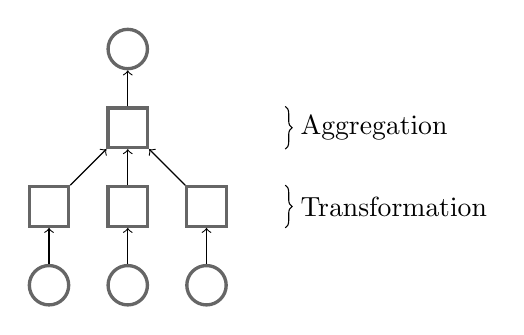
\begin{tikzpicture}[
        layer/.style={rectangle, draw=black!60, fill=white, very thick, minimum size=5mm},
        inout/.style={circle, draw=black!60, fill=white, very thick, minimum size=5mm},
        layergroup/.style={decorate},
        tubnode/.style={midway, right=2pt},
        ]
        \node[inout] (OUT)              {}; 
        \node[layer] (AGG) [below of=OUT] {}; 
        \node[layer] (TR2) [below of=AGG] {}; 
        \node[layer] (TR1) [left of=TR2] {}; 
        \node[layer] (TR3) [right of=TR2] {}; 
        \node[inout] (IN1) [below of=TR1] {}; 
        \node[inout] (IN2) [below of=TR2] {}; 
        \node[inout] (IN3) [below of=TR3] {}; 
        \draw[->] (AGG) -- (OUT);
        \draw[->] (TR1) -- (AGG); 
        \draw[->] (TR2) -- (AGG); 
        \draw[->] (TR3) -- (AGG); 
        \draw[->] (IN1) -- (TR1); 
        \draw[->] (IN2) -- (TR2); 
        \draw[->] (IN3) -- (TR3);
        \draw[layergroup, decoration={brace}] let \p1=(AGG.north), \p2=(AGG.south) in
        ($(2, \y1)$) -- ($(2, \y2)$) node[tubnode] {Aggregation};
        \draw[layergroup, decoration={brace}] let \p1=(TR2.north), \p2=(TR2.south) in
        ($(2, \y1)$) -- ($(2, \y2)$) node[tubnode] {Transformation};    
    \end{tikzpicture}
    \caption{A simple GNN}
\end{figure*}

In both the aggregation and transformation layers, we could include a 3-layer MLP.  

\subsubsection{Adding non-message passing layers}

We can add pre- and postprocessing layers. 

\begin{figure*}[ht]
    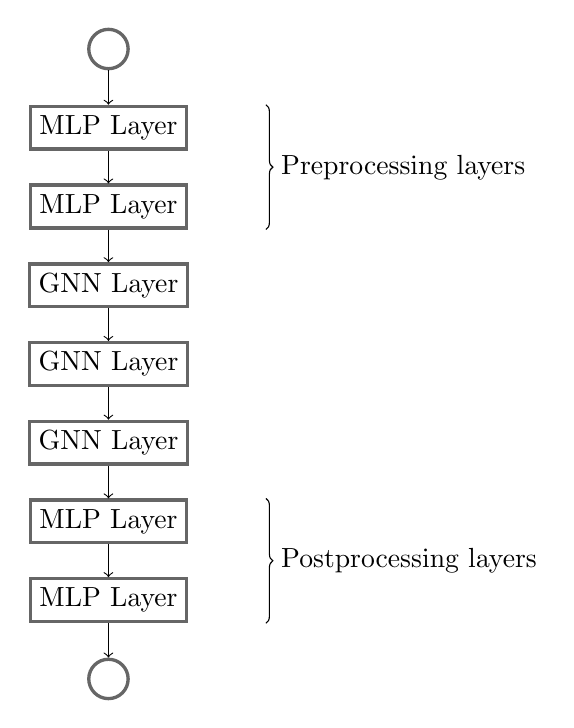
\begin{tikzpicture}[
        layer/.style={rectangle, draw=black!60, fill=white, very thick, minimum size=5mm},
        layergroup/.style={decorate},
        tubnode/.style={midway, right=2pt},
        inout/.style={circle, draw=black!60, fill=white, very thick, minimum size=5mm},
        ]
        \node[inout] (IN)                   {}; 
        \node[layer] (MLP1) [below of=IN]   {MLP Layer}; 
        \node[layer] (MLP2) [below of=MLP1] {MLP Layer}; 
        \node[layer] (GNN3) [below of=MLP2] {GNN Layer}; 
        \node[layer] (GNN4) [below of=GNN3] {GNN Layer}; 
        \node[layer] (GNN5) [below of=GNN4] {GNN Layer}; 
        \node[layer] (MLP6) [below of=GNN5] {MLP Layer}; 
        \node[layer] (MLP7) [below of=MLP6] {MLP Layer}; 
        \node[inout] (OUT)  [below of=MLP7] {}; 
        \draw[->] (IN) -- (MLP1); 
        \draw[->] (MLP1) -- (MLP2); 
        \draw[->] (MLP2) -- (GNN3); 
        \draw[->] (GNN3) -- (GNN4); 
        \draw[->] (GNN4) -- (GNN5); 
        \draw[->] (GNN5) -- (MLP6); 
        \draw[->] (MLP6) -- (MLP7); 
        \draw[->] (MLP7) -- (OUT); 
        \draw[layergroup, decoration={brace}] let \p1=(MLP1.north), \p2=(MLP2.south) in
        ($(2, \y1)$) -- ($(2, \y2)$) node[tubnode] {Preprocessing layers};
        \draw[layergroup, decoration={brace}] let \p1=(MLP6.north), \p2=(MLP7.south) in
        ($(2, \y1)$) -- ($(2, \y2)$) node[tubnode] {Postprocessing layers};
        %\twoup{MLP1}{MLP2}{Preprocessing layers};
        %\threeup{GNN3}{GNN4}{GNN5}{group};
        %\twoup{MLP6}{MLP7}{Preprocessing layers};
    
    \end{tikzpicture}
    \caption{A simple GNN}
\end{figure*}

These MLP layers refine the features of the nodes before and after the GNN layers. The preprocessing layers could process note features, for instance, if the nodes represent images or text. The postprocessing layers could process the embedding, for instance, if we want to use the embedding as a feature for classification.
    
\subsubsection{Skip Connections}
Skip the layers in the neural Network

\begin{figure*}[ht]
    \begin{tikzpicture}[
        layer/.style={rectangle, draw=black, fill=white, very thick, minimum size=5mm},
        layergroup/.style={decorate},
        tubnode/.style={midway, right=2pt},
        inout/.style={circle, draw=black, fill=white, very thick, minimum size=5mm},
        silent/.style={circle,fill=black,minimum size=1pt}
        ]
        \node[inout]  (IN)                     {};
        \node[layer]  (MLP11) [below of=IN]    {MLP Layer};
        \node[layer]  (MLP12) [below of=MLP11] {MLP Layer};
        \node[silent] (S1)    [below of=MLP12] {};
        \node[layer]  (GNN1)  [below of=S1]    {GNN Layer}; 
        \node[silent] (S2)    [below of=GNN1]  {};
        \node[layer]  (GNN2)  [below of=S2]    {GNN Layer};
        \node[silent] (S3)    [below of=GNN2]  {};
        \node[layer]  (GNN3)  [below of=S3]    {GNN Layer}; 
        \node[silent] (S4)    [below of=GNN3]  {};
        \node[layer]  (MLP21) [below of=S4]    {MLP Layer}; 
        \node[layer]  (MLP22) [below of=MLP21] {MLP Layer}; 
        \node[inout]  (OUT)   [below of=MLP22  {}; 
        \draw[->] (IN) -- (MLP11); 
        \draw[->] (MLP11) -- (MLP12); 
        \draw[->] (MLP12) -- (S1); 
        \draw[->] (S1) -- (GNN1); 
        %\draw[->] (MLP2) -- (GNN4);
        %\draw (S1) to [out=-180,in=180,looseness=1.5] (GNN3); 
        \draw[->] (GNN1) -- (S2); 
        \draw[->] (S2) -- (GNN2);
        \draw[->] (GNN2) -- (S3); 
        \draw[->] (S3) -- (GNN3);
        \draw[->] (GNN3) -- (MLP21);
        \draw[->] (MLP21) -- (MLP22); 
        \draw[->] (MLP22) -- (OUT); 
        \draw[layergroup, decoration={brace}] let \p1=(MLP1.north), \p2=(MLP2.south) in
        ($(2, \y1)$) -- ($(2, \y2)$) node[tubnode] {Preprocessing layers};
        \draw[layergroup, decoration={brace}] let \p1=(MLP6.north), \p2=(MLP7.south) in
        ($(2, \y1)$) -- ($(2, \y2)$) node[tubnode] {Postprocessing layers};
        %\twoup{MLP1}{MLP2}{Preprocessing layers};
        %\threeup{GNN3}{GNN4}{GNN5}{group};
        %\twoup{MLP6}{MLP7}{Preprocessing layers};
    
    \end{tikzpicture}
    \caption{A simple GNN with skipping}
\end{figure*}


% \begin{tikzpicture}[node distance={15mm}, thick, main/.style = {draw, circle}] 
% \node[main] (1) {$x_1$}; 
% \node[main] (2) [above right of=1] {$x_2$}; 
% \node[main] (3) [below right of=1] {$x_3$}; 
% \node[main] (4) [above right of=3] {$x_4$}; 
% \node[main] (5) [above right of=4] {$x_5$}; 
% \node[main] (6) [below right of=4] {$x_6$}; 
% \draw[->] (1) -- (2); 
% \draw[->] (1) -- (3); 
% \draw (1) to [out=135,in=90,looseness=1.5] (5); 
% \draw (1) to [out=180,in=270,looseness=5] (1); 
% \draw (2) -- (4); 
% \draw (3) -- (4); 
% \draw (5) -- (4); 
% \draw[->] (5) to [out=315, in=315, looseness=2.5] (3); 
% \draw[->] (6) -- node[midway, above right, sloped, pos=1] {+1} (4); 
% \end{tikzpicture} 
 
 

\begin{thebibliography}{10}

  \bibitem{grovlesk16} Grover and Leskovovec, 
  \emph{???}, 2016.
  
  \bibitem{latexMath} Graetzer George, \emph{Math Into \LaTeX},
  Birkuser Boston; 3 edition (June 22, 2000).
  
\end{thebibliography}
  
\end{document}
